%!TEX root = head-full.tex

\section{Metropolis-Hastings} \label{sec:metropolis_hastings}
In the Introduction, we have shown the main idea of an MCMC sampling method. In this section, we will introduce the Metropolis Hastings Algorithm and conduct an experiment.



\subsection{Algorithm\protect\footnote{Available at \protect\url{https://github.com/lzhbrian/MCMC/blob/master/src/MH/metropolis_hasting.R} in R\cite{R}}}

\subsubsection{Detailed Balance Condition}
Before stepping further into the MH Algorithm, We would first introduce a theorem called the Detailed Balance Condition. 

In the introduction, we said that we want to construct a Markov Chain which its stationary distribution $\pi(x)$ just equals to the required probability distribution $p(x)$.

At first, a theorem is needed.
\begin{theorem}[Detail Balance Condition] \label{theo:detail_balance_condition}
Given a non periodic Markov Chain, if 
\begin{equation} 
\pi(i) P_{ij} = \pi(j) P_{ji}~~for~all~i,j 
\end{equation}
then $\pi(x)$ is the stationary distribution of this Markov Chain.
\end{theorem}
So, the key question will be how to construct a Markov Chain which satisfy this Detail Balance Condition.

\subsubsection{MCMC sampling method}
Suppose we already have a transition matrix $Q$ for a Markov Chain, $q(i,j)$ denote the probabilty of transition from state $i$ to state $j$. For the general case, 
$$p(i) q(i,j) \neq p(j) q(j,i)$$
That is to say, we do not have the detailed balance condition (Theorem~\ref{theo:detail_balance_condition})
So we introduce an $\alpha(i,j)$ s.t.
\begin{equation} 
p(i) q(i,j)\alpha(i,j) = p(j) q(j,i)\alpha(j,i) 
\end{equation}
By sysmetrical characteristic, we choose:
\begin{equation} 
\alpha(i,j)= p(j) q(j,i), \quad \alpha(j,i) = p(i) q(i,j)
\end{equation}
So the new Markov Chain $Q'$ would have the property of which its stationary distribution is $p(x)$
\begin{equation}
\label{detailed-balance} 
p(i) \underbrace{q(i,j)\alpha(i,j)}_{Q'(i,j)} 
= p(j) \underbrace{q(j,i)\alpha(j,i)}_{Q'(j,i)}
\end{equation}

We call the $\alpha(i,j)$ we introduced, accepting ratio. It means that, in the original Markov Chain $Q$, when state $i$ transits to state $j$ with a probability of $q(i,j)$, we accept this transition with a probabilty of $\alpha(i,j)$

Now, we have derived the MCMC sampling method.

\subsubsection{Metropolis-Hastings Algorithm}
The MCMC sampling method is a marvellous work. However, it has a critical drawback that if $\alpha(i,j)$ \& $\alpha(j,i)$ are too small, we would seldom accept the transition.

A solution is that we multiply both $\alpha(i,j)$ \& $\alpha(j,i)$ with a constant to make sure that the larger one between them equals $1$. By doing so, we change the accepting ratio to
\begin{equation}
\alpha(i,j) = \min\left\{\frac{p(j)q(j,i)}{p(i)q(i,j)},1\right\}
\end{equation}
and now, we get Metropolis-Hastings Algorithm\cite{hastings1970monte}.

I would like to further introduce one more concept called accepting rate(not accepting ratio), which denotes the statistic ratio of accepting the transition. i.e. If we request 10 transition and we accept 8 times, then the accepting rate would be 0.8. This concept is crucial when we are dealing with a continual Markov Chain to use the MH algorithm.



\subsubsection{Symmetric Case}
In a Markov Chain whose transition matrix is symmetric, we have
$$q(i,j)=q(j,i)$$
so the accepting ratio could be simplified to 
\begin{equation}
\alpha(i,j) = \min\left\{\frac{p(j)}{p(i)},1\right\}
\end{equation}
which is also known as the Metropolis Algorithm\cite{metropolis1953equation}.

\subsubsection{Continual Case}
In a continual Markov Chain, such as the experiment we are going to do in the next subsection, we have a vague definition of transition matrix $Q$. So we introduce a concept called the proposal jump size, $sd.T$.

The method we get $x_{k+1}$ from $x_{k}$ is to add a sampled point of a normal distribution with a variance of the jump size and $\mu=0$. For a two dimension example, we have:
\begin{equation}
x_{k+1} = x_{k} + sd.T \left( \begin{array}{ccc}
n_{1} \\
n_{2} \end{array} \right) 
\end{equation}

	\begin{algorithm}
        \caption{Metropolis-Hastings}
        \begin{algorithmic}
        	\Require Required distribution $p$, Transfer Matrix $Q$
        	\State Initialize $x_{1}$ 
            \For{$t = 1 \to \inf$}
                \State Sample $y \sim q(x|x_{t})$
	            \State Sample $u \sim U{[0,1]}$
	            \If {$u < \alpha(x_{t},y)=min\{\frac{p(y)q(x_{t}|y)}{p(x_{t})q(y|x_{t})},1\}$}
	                \State $x_{t+1} \gets y$
	            \Else
	            	\State $x_{t+1} \gets x_{t}$
	            \EndIf
			\EndFor
        \end{algorithmic}
    \end{algorithm}




\subsection{Sampling Experiment}
For our experiment, we use an example of a bivariate Normal distribution, with
$$ \mu = \left( \begin{array}{ccc}
5 \\
10 \end{array} \right), 
\Sigma = \left( \begin{array}{ccc}
1 & 1\\
1 & 4\end{array} \right)$$

By theoretical computation, we can easily compute the the pearson correlation between the two dimensional value is 0.5.
$$ \rho = 0.5 $$

We then generate 10,000 samples using the MH algorithm and take the second half (i.e. the last 5,000 points), setting the standard deviation of proposal to 3.0. We can see from the result (Figure~\ref{fig:sample_result}) that we have derived 5,000 sampled points whose pearson correlation value $\rho=0.50009$, which matches the theoretical value.

\begin{figure}[tb]
\vspace{-0.5in}
  	\centering
  	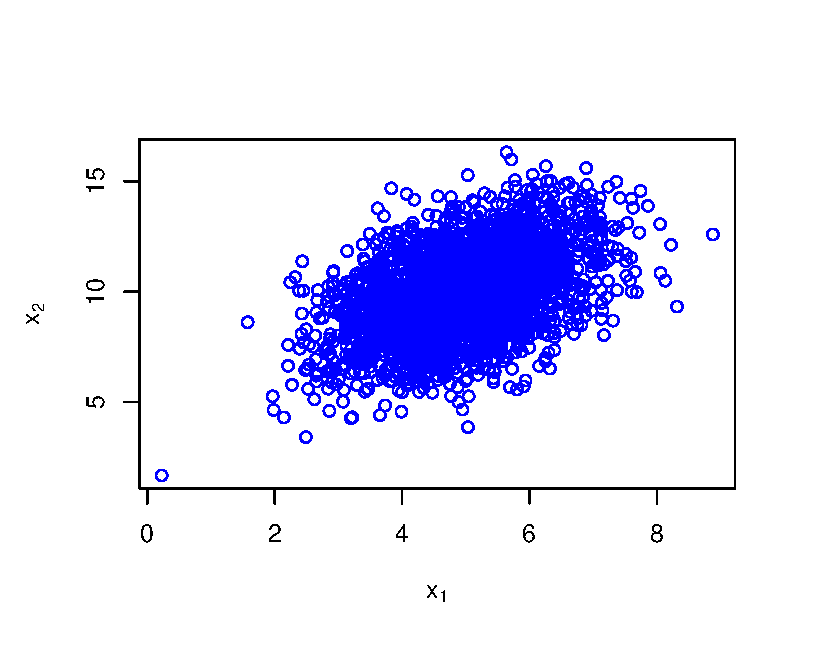
\includegraphics[width=0.4\textwidth]{figure/sample_result.eps}
\vspace{-0.2in}
	\caption{Sampling result of 5,000 points \protect\\ correlation = 0.50009 , set sd.T = 3.0}
	\label{fig:sample_result}
\end{figure}




\subsection{Performance Analysis}

\subsubsection{Choice of proposal jump size}
MH algorithm is an effective MCMC method for many diverse problems. However, for a continual case in MH algorithm, its performance somewhat depends on the selection of the proposal density. With the proposal jump size being small, the accepting rate would be very low and eventually stick to only one point(eg. the initial point); When the proposal jump size is too big, the accepting rate would be too high. 

Roberts et al. have shown in previous work\cite{roberts1997weak} that the optimal accepting rate of the MH algorithm should approximately be at 0.234 for the case of an N-dimensional Gaussian target distribution. We test the accepting rates in different proposal jump size(Figure~\ref{fig:acc_sdt}) and find that the optimal value should be at appoximately 3.0 to acquire a model with accepting rate being close to 0.234. That is the reason why we choose 3.0 as our proposal jump size.

\begin{figure}[tb]
\vspace{-0.2in}
  	\centering
  	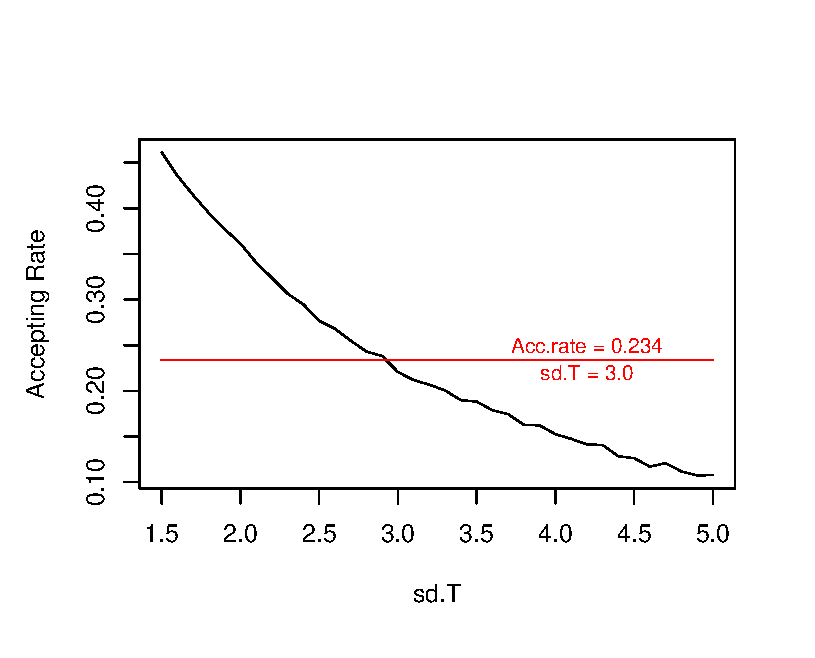
\includegraphics[width=0.4\textwidth]{figure/acc_sdt.eps}
\vspace{-0.2in}
	\caption{Accepting rate on different proposal jump size.}
	\label{fig:acc_sdt}
\end{figure}

\subsubsection{Efficiency}
Due to the limit of the accepting rate, for a high dimensional condition, using the MH sampling methods may spend more time in traverse all of the possible states, which could sometimes be be less satisfying. Thus, many would switch to Gibbs Sampling Algorithm.




\subsection{Gibbs Sampling}
Gibbs Sampling is a special case of Metropolis Hastings Algorithm, by letting the accepting rate = 1, we will get a Gibbs Sampler. As the length \& time limit, we will not specify more here.
But it is worthy to notice that Gibbs sampling method is used more often than Metropolis-Hastings method in the real practice, probably because it has a slightly simpler process.






